\documentclass[10pt,a4paper]{article}
\usepackage[utf8]{inputenc}
\usepackage[german]{babel}
\usepackage[T1]{fontenc}
\usepackage{amsmath}
\usepackage{amsfonts}
\usepackage{amssymb}
\usepackage{graphicx}
\usepackage[left=2cm,right=2cm,top=2cm,bottom=2cm]{geometry}
\title{Einführung in die Neuroinformatik}

%\newcommand{\Name}[Anzahl]{Definition}
\newcommand{\termin}[3]{\section{Termin #1} \bf(Seiten: #2 - #3)\\}

%\newenvironment{NAME}[ANAZHL][OPTIONAL]{BEGIN}{END}
\newenvironment{merk}[1]{\noindent\makebox[\linewidth]{\rule{\textwidth}{0.2pt}}\\\bf Seite: #1\\ \bf Anmerkung: \\ \\}{}


\begin{document}
\maketitle

%Vorlesungsaufschreibe
\termin{20180424}{31}{52}
% ################## Anmerkung ############################# %
 \begin{merk}{43}

n Neuronen

\begin{figure}[htbp]
    \begin{center}
        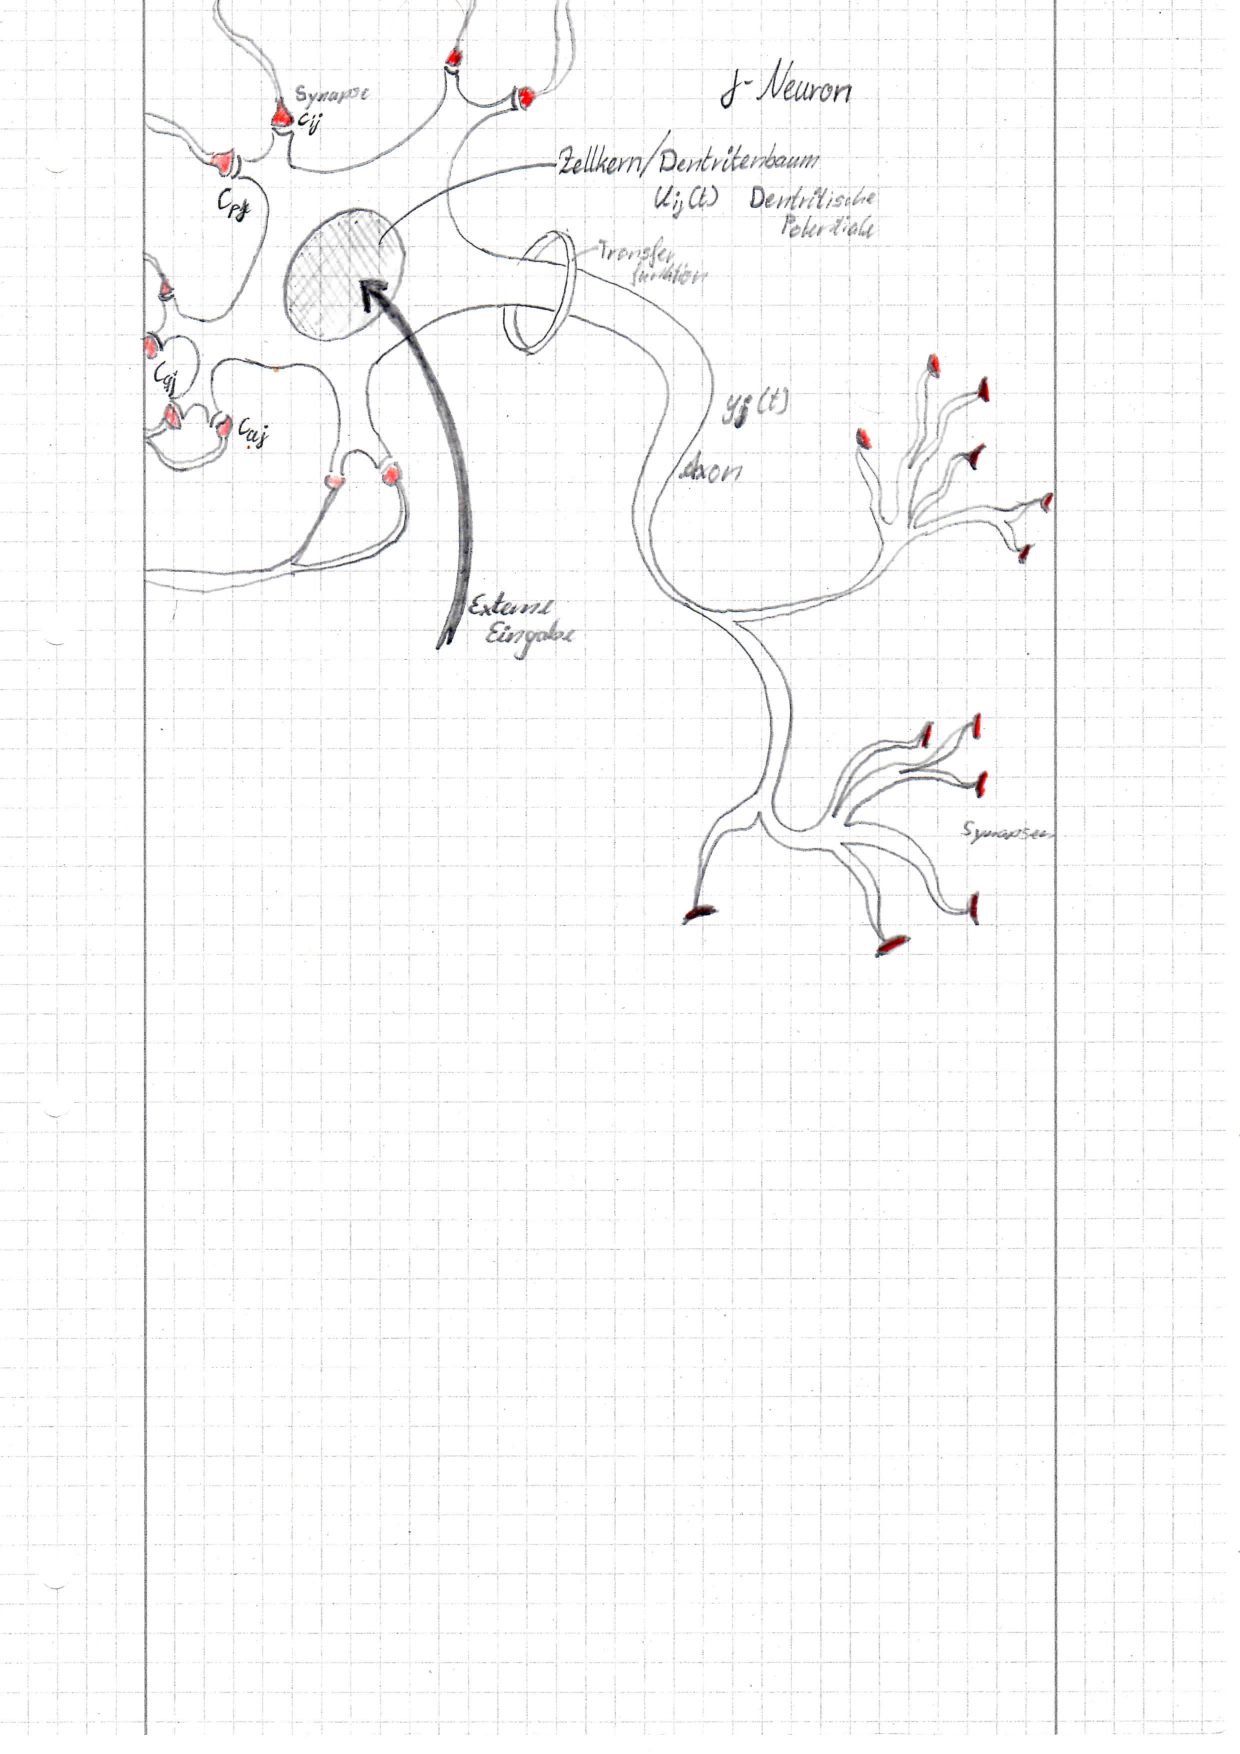
\includegraphics[trim=70 350 70 0, clip, width=.7\textwidth, height=200px]{img_0001.pdf}
    \caption{$img\_0001$}
    \label{img_0001}
    \end{center}
\end{figure}

[ \r{u} = Zeitlich integriert]\\
\begin{center}

$$ \dot u_j(t) = \lim_{t \to t_n} \frac{ u_i(t_0) - u_j(t) } { t_0 - t } $$

$$\dot u_j(t) =  - u_j(t) + \underbrace{ \sum_{i=1}^n ( c_{i,j} * y_i^{ t - d_{i,j} }) + x_j(t)}_{e_j(t)}$$

$$ \tau \r{u} = - u  $$
     $$   = u(t) = e^(\frac{-t}{\tau})$$
$$\tau > 0$$

\end{center}
\newpage
\begin{figure}[htbp]
    \begin{center}
        \includegraphics[width=.7\textwidth, keepaspectratio, page=3]{img_0002_0004.pdf}
    \caption{$ img\_0002\_0004$}
    \label{img_0002_0004}
    \end{center}
\end{figure}
\begin{center}
$$ \dot{u} = - u , u(t) = e^{-t}$$
\end{center}

\begin{figure}[htbp]
    \begin{center}
        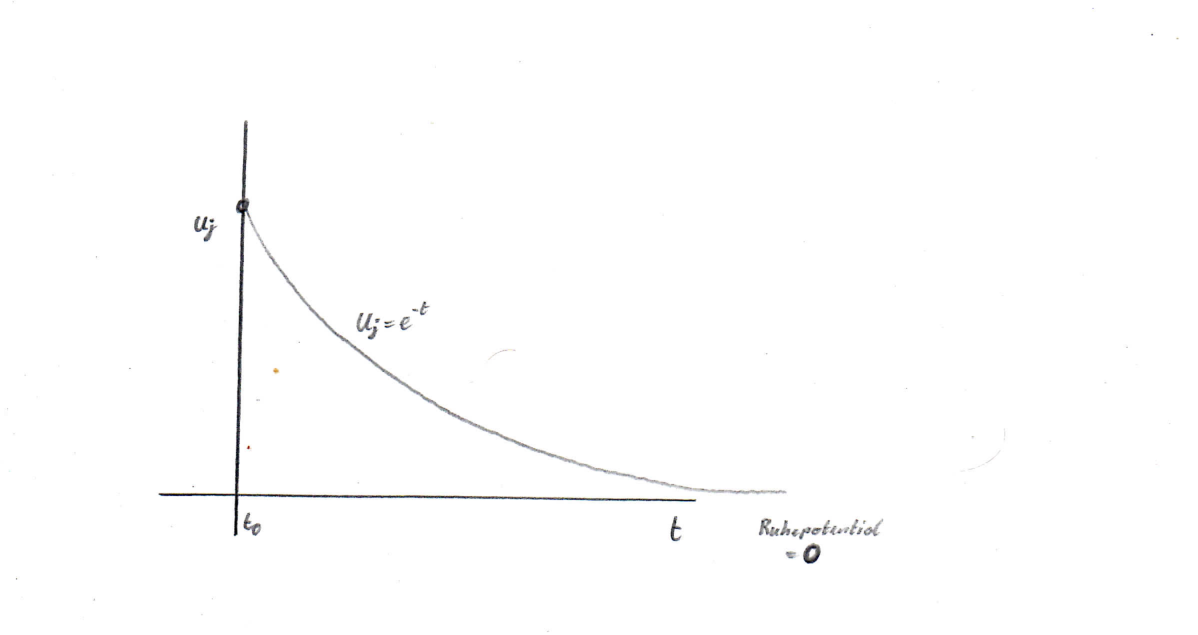
\includegraphics[width=.7\textwidth, keepaspectratio, page=1]{img_0002_0004.pdf}
    \caption{$ img\_0002\_0004$}
    \label{img_0002_0004}
    \end{center}
\end{figure}
\end{merk}



% ################## Anmerkung ############################# %
\begin{merk}{44}
$\rho = \text{\ Gedächtnisvariable} $\\
Wird in unseren Berechnungen meist vernachlässigt und auf 1 gesetzt.\\
Wir werden kein Gedächtnis einbauen.

\end{merk}
\newpage
% ################## Anmerkung ############################# %
\begin{merk}{45}
\begin{figure}[htbp]
    \begin{center}
        \includegraphics[width=.7\textwidth, keepaspectratio, page=2]{img_0002_0004.pdf}
    \caption{$ img\_0002\_0004$}
    \label{img_0002_0004}
    \end{center}
\end{figure}
\end{merk}


\end{document}